\documentclass{standalone}
\usepackage{tikz}

\begin{document}
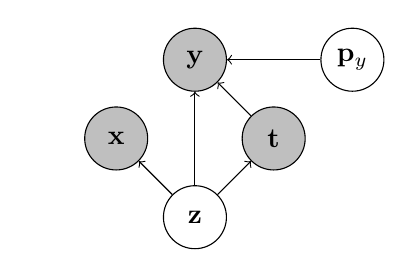
\begin{tikzpicture}
    \node[circle, draw=black, fill=lightgray, minimum size=0.8cm] (t) at (2, 1) {$\mathbf{t}$};
    \node[circle, draw=black, fill=lightgray, minimum size=0.8cm] (y) at (1, 2) {$\mathbf{y}$};
    \node[circle, draw=black, fill=white, minimum size=0.8cm] (z) at (1, 0) {$\mathbf{z}$};
    \node[circle, draw=black, fill=lightgray, minimum size=0.8cm] (x) at (0, 1) {$\mathbf{x}$};
    \node[circle, draw=black, fill=white, minimum size=0.8cm] (yp) at (3, 2) {$\mathbf{p}_{y}$};
    \node[draw=white] (none) at (-1, 2) {};

    
    \draw[->] (z) -- (x);
    \draw[->] (z) -- (y);
    \draw[->] (z) -- (t);
    \draw[->] (t) -- (y);
    \draw[->] (yp) -- (y);
\end{tikzpicture}
\end{document}